\chapter{Der Fall Lena}\label{ch:fall_lena}

Lena ist 13 Jahre alt und geht in die 1.~Klasse eines Gymnasiums.
An einem Montagmorgen ist alles anders:

\begin{itemize}
	\item Auf ihrem Social-Media-Konto erscheinen Beiträge, die sie nie geschrieben hat. Ihr Passwort funktioniert nicht mehr.
	\item Ein Unbekannter schreibt ihr: \enquote{Schöner Garten übrigens. Wohnst du nicht an der Bahnhofstrasse?}
	\item Im Klassenchat macht ein Meme die Runde: ein Foto von Lena, wie sie im Schullager mit offenem Mund schläft.
\end{itemize}

\begin{figure}[H]
	\centering
	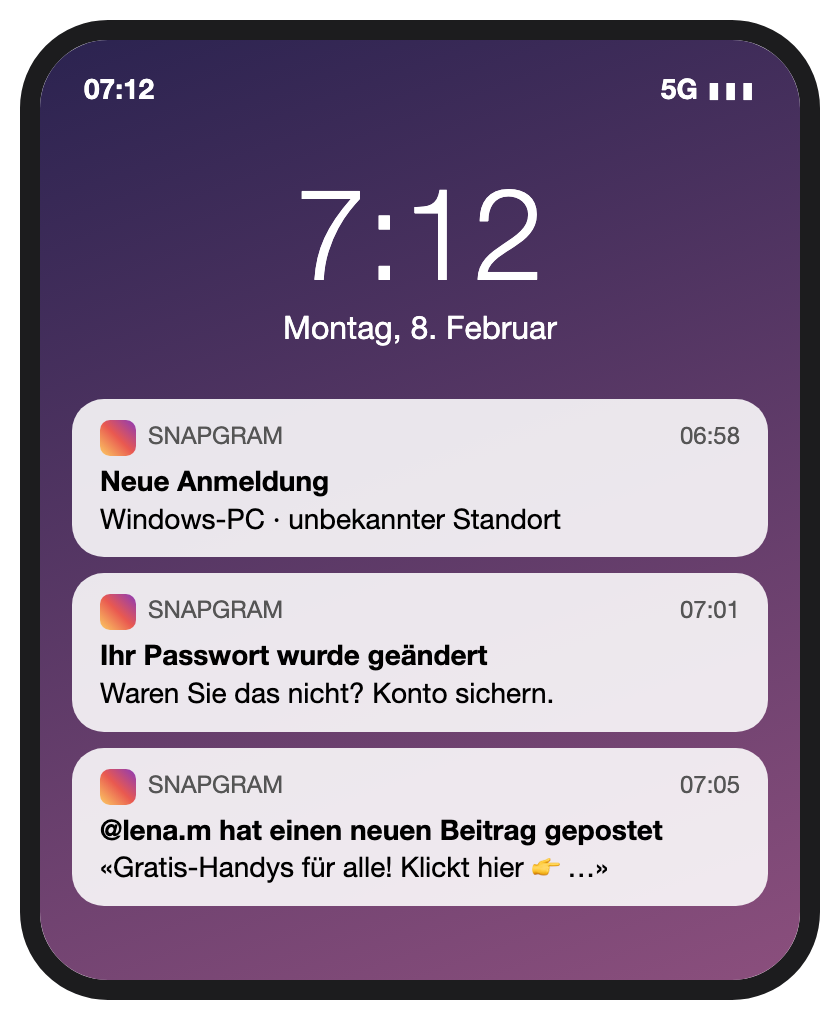
\includegraphics[height=5.6cm,keepaspectratio]{Medienkompetenzwoche/UG_Datenschutz/Figures/lena_1_gehackt}\hfill
	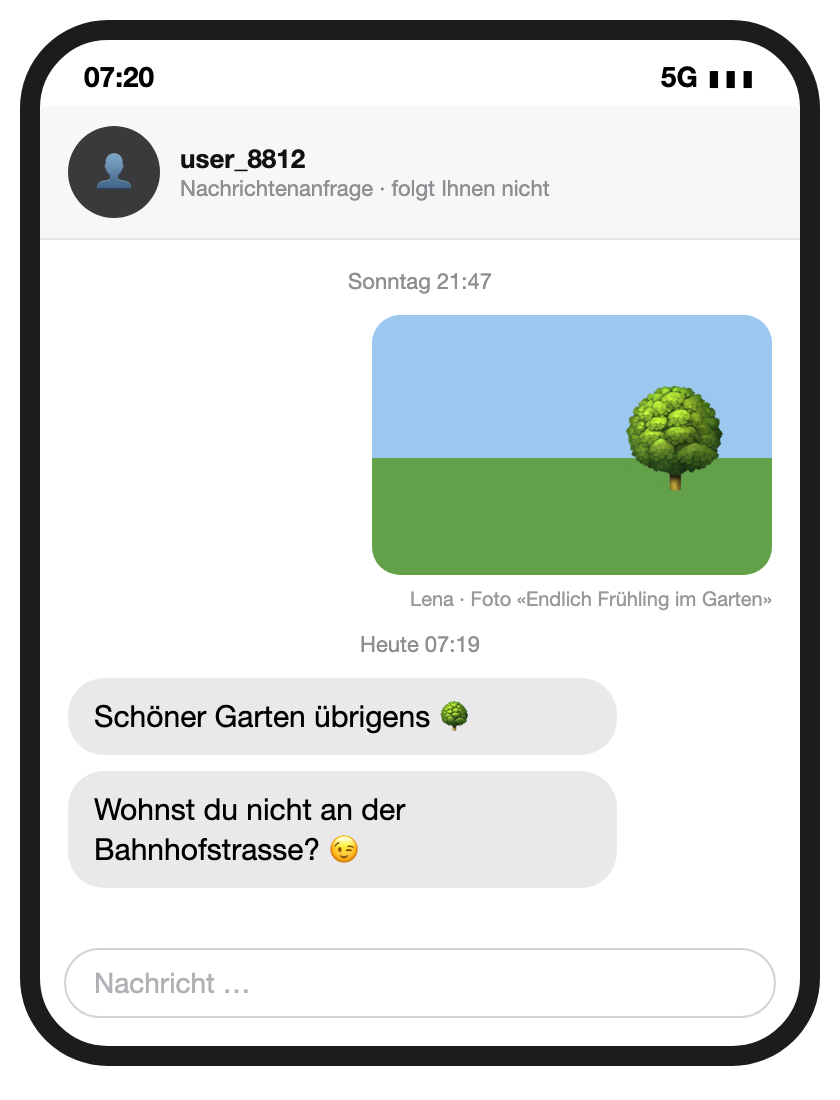
\includegraphics[height=5.6cm,keepaspectratio]{Medienkompetenzwoche/UG_Datenschutz/Figures/lena_2_nachricht}\hfill
	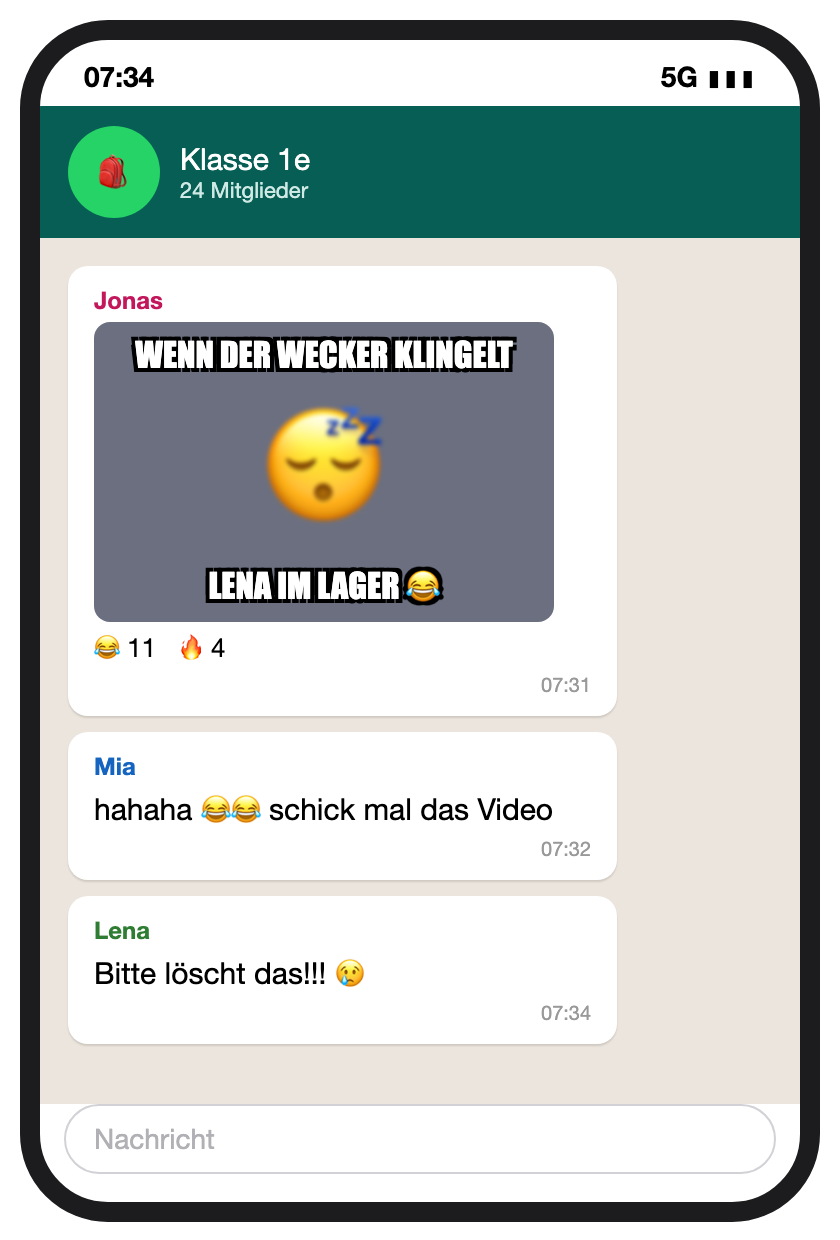
\includegraphics[height=5.6cm,keepaspectratio]{Medienkompetenzwoche/UG_Datenschutz/Figures/lena_3_klassenchat}
	\caption{Lenas Handy am Montagmorgen (nachgestellte Bildschirme, alle Namen und Dienste sind erfunden).}
	\label{fig:lena_handy}
\end{figure}

Lena versteht die Welt nicht mehr. Sie hat doch nichts Verbotenes getan -- oder doch?

\begin{myremark}
	Heute ermitteln Sie in diesem Fall. An drei Stationen finden Sie heraus,
	\textbf{wie} es dazu kommen konnte und \textbf{was} Lena (und Sie) dagegen tun können.
	Am Ende lösen Sie den Fall und erstellen ein eigenes Produkt.
\end{myremark}

\section{Ihre Lernziele}

Am Ende dieses Halbtags können Sie \dots
\begin{enumerate}
	\item erklären, welche Daten Fotos, Apps und Geräte über Sie verraten, und die wichtigsten Einstellungen auf Ihrem Handy gezielt anpassen;
	\item ein sicheres Passwort bilden, die Gefahr von wiederverwendeten Passwörtern erklären und eine Phishing-Nachricht an mindestens drei Merkmalen erkennen;
	\item an Beispielen begründet entscheiden, ob Sie ein Bild oder Video veröffentlichen dürfen, und ein frei lizenziertes Bild korrekt angeben.
\end{enumerate}

\section{So arbeiten Sie heute}

\begin{myprocedure}[Ablauf des Lernateliers]
	\begin{enumerate}
		\item \textbf{Einstieg (gemeinsam):} Die Lehrperson stellt den Fall vor und zeigt ein kurzes Experiment.
		\item \textbf{Lernatelier (zu zweit):} Sie bearbeiten die drei Stationen A, B und C in der Reihenfolge, die Ihnen die Lehrperson zuteilt. Pro Station haben Sie etwa 30--35 Minuten Zeit.
		\item \textbf{Fall lösen und Produkt (zu zweit):} Sie tragen Ihre Erkenntnisse zusammen und erstellen ein Produkt (\cref{ch:produkt}).
		\item \textbf{Abschluss (gemeinsam):} Galerie der Produkte und Auflösung des Falls.
	\end{enumerate}
\end{myprocedure}

\begin{myattention}
	\begin{itemize}
		\item Sie arbeiten teilweise mit Ihrem eigenen Handy. \textbf{Zeigen Sie niemandem private Fotos oder Nachrichten}, und schauen Sie nicht auf fremde Bildschirme.
		\item Geben Sie auf Webseiten \textbf{nie echte Passwörter} ein -- auch nicht auf Testseiten.
		\item \textbf{Pflichtaufgaben} (blau) bearbeiten alle. \textbf{Challenges} (gelb) sind für Teams, die schneller vorankommen.
		\item Wenn Sie nicht weiterkommen: zuerst im Team überlegen, dann ein anderes Team fragen, dann die Lehrperson.
	\end{itemize}
\end{myattention}

\section{Laufzettel}

Haken Sie ab, was Sie erledigt haben. So behalten Sie und die Lehrperson den Überblick.

\begin{center}
	\renewcommand{\arraystretch}{1.4}
	\begin{tabular}{lp{7.2cm}cc}
		\textbf{Station}                          & \textbf{Thema}                                & \textbf{Pflicht}       & \textbf{Challenge}     \\
		\midrule
		A (\cref{ch:spurensuche})                 & Spurensuche: Was verraten Fotos und Geräte?   & \faSquare[regular]     & \faSquare[regular]     \\
		B (\cref{ch:tatort_konto})                & Tatort Konto: Passwörter und Phishing         & \faSquare[regular]     & \faSquare[regular]     \\
		C (\cref{ch:posten})                      & Darf ich das posten?                          & \faSquare[regular]     & \faSquare[regular]     \\
		\midrule
		Fallakte (\cref{sec:fall_loesen})         & Fall Lena lösen                               & \faSquare[regular]     &                        \\
		Produkt (\cref{sec:produkt_waehlen})      & Entscheidungsbaum oder Phishing-Falle         & \faSquare[regular]     &                        \\
	\end{tabular}
\end{center}
